\begin{figure}[H]
	\centering
	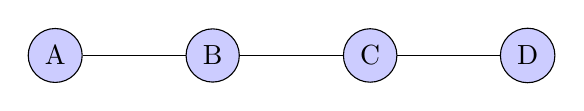
\begin{tikzpicture}
		\node[circle, draw, fill=blue!20] (A) at (0,0) {A};
		\node[circle, draw, fill=blue!20] (B) at (2,0) {B};
		\node[circle, draw, fill=blue!20] (C) at (4,0) {C};
		\node[circle, draw, fill=blue!20] (D) at (6,0) {D};
		
		\draw (A) -- (B);
		\draw (B) -- (C);
		\draw (C) -- (D);
	\end{tikzpicture}
	\caption{Graph diameter example showing the longest shortest path A-B-C-D with diameter 3.}
	\label{fig:graph-diameter-example}
\end{figure}
